\documentclass[]{article}
\usepackage{float}
\usepackage{graphicx}
\usepackage[svgnames]{xcolor} 
\usepackage{fancyhdr}
\usepackage{fancyvrb}
\usepackage{forest}
\usepackage{tocloft}
\usepackage[hidelinks]{hyperref}
\usepackage{enumitem}
\usepackage[many]{tcolorbox}
\usepackage{listings }
\usepackage[a4paper, total={6in, 8in} , top = 2cm,bottom = 4cm]{geometry}
%\usepackage[a4paper, total={6in, 8in}]{geometry}
\usepackage{afterpage}
\usepackage{amssymb}
\usepackage{pdflscape}
\usepackage{textcomp}
\usepackage{xecolor}
\usepackage{rotating}
\usepackage[Kashida]{xepersian}
\usepackage[T1]{fontenc}
\usepackage{tikz}
\usepackage[utf8]{inputenc}
\usepackage{PTSerif} 
\usepackage{seqsplit}
\usepackage{changepage}


\usepackage{listings}
\usepackage{xcolor}
\usepackage{sectsty}

\setcounter{secnumdepth}{0}
 
\definecolor{codegreen}{rgb}{0,0.6,0}
\definecolor{codegray}{rgb}{0.5,0.5,0.5}
\definecolor{codepurple}{rgb}{0.58,0,0.82}
\definecolor{backcolour}{rgb}{0.95,0.95,0.92}
\definecolor{blanchedalmond}{rgb}{1.0, 0.92, 0.8}
\definecolor{brilliantlavender}{rgb}{0.96, 0.73, 1.0}
 
\NewDocumentCommand{\codeword}{v}{
\texttt{\textcolor{blue}{#1}}
}
\lstset{language=java,keywordstyle={\bfseries \color{blue}}}

\lstdefinestyle{mystyle}{
    backgroundcolor=\color{backcolour},   
    commentstyle=\color{codegreen},
    keywordstyle=\color{magenta},
    numberstyle=\tiny\color{codegray},
    stringstyle=\color{codepurple},
    basicstyle=\ttfamily\normalsize,
    breakatwhitespace=false,         
    breaklines=true,                 
    captionpos=b,                    
    keepspaces=true,                 
    numbers=left,                    
    numbersep=5pt,                  
    showspaces=false,                
    showstringspaces=false,
    showtabs=false,                  
    tabsize=2
}

\lstset{style=mystyle}

\settextfont[BoldFont={XB Zar bold.ttf}]{XB Zar.ttf}

\setlatintextfont[Scale=1.0,
 BoldFont={LiberationSerif-Bold.ttf}, 
 ItalicFont={LiberationSerif-Italic.ttf}]{LiberationSerif-Regular.ttf}


\newfontfamily{\mymono}{[JetBrainsMono-Medium.ttf]}


\newcommand{\inputsample}[1]{
    ~\\
    \textbf{ورودی نمونه}
    ~\\
    \begin{tcolorbox}[breakable,boxrule=0pt]
        \begin{latin}
            \large{
                #1
            }
        \end{latin}
    \end{tcolorbox}
}

\newcommand{\outputsample}[1]{
    ~\\
    \textbf{خروجی نمونه}

    \begin{tcolorbox}[breakable,boxrule=0pt]
        \begin{latin}
            \large{
                #1
            }
        \end{latin}
    \end{tcolorbox}
}

\newtcolorbox{mybox}[2][]{colback=red!5!white,
colframe=red!75!black,fonttitle=\bfseries,
colbacktitle=red!85!black,enhanced,
attach boxed title to top center={yshift=-2mm},
title=#2,#1}

\newenvironment{changemargin}[2]{%
\begin{list}{}{%
\setlength{\topsep}{0pt}%
\setlength{\leftmargin}{#1}%
\setlength{\rightmargin}{#2}%
\setlength{\listparindent}{\parindent}%
\setlength{\itemindent}{\parindent}%
\setlength{\parsep}{\parskip}%
}%
\item[]}{\end{list}}


\definecolor{foldercolor}{RGB}{124,166,198}
\definecolor{sectionColor}{HTML}{ff5e0e}
\definecolor{subsectionColor}{HTML}{008575}

\definecolor{listColor}{HTML}{00d3b9}

\definecolor{umlrelcolor}{HTML}{3c78d8}

\definecolor{subsubsectionColor}{HTML}{3c78d8}

\defpersianfont\authorFont[Scale=0.9]{XB Zar bold.ttf}

\defpersianfont\titr[Scale=1.5]{Lalezar-Regular.ttf}

\defpersianfont\fehrest[Scale=1.2]{Lalezar-Regular.ttf}

\defpersianfont\fehrestTitle[Scale=3.0]{Lalezar-Regular.ttf}

\defpersianfont\fehrestContent[Scale=1.2]{XB Zar bold.ttf}

\sectionfont{\color{sectionColor}}  % sets colour of sections
\subsectionfont{\color{subsectionColor}}  % sets colour of sections
\subsubsectionfont{\color{subsubsectionColor}}


\renewcommand{\labelitemii}{$\circ$}


\renewcommand{\baselinestretch}{1.1}


\renewcommand{\contentsname}{فهرست}

\renewcommand{\cfttoctitlefont}{\fehrestTitle}


\renewcommand\cftsecfont{\color{sectionColor}\fehrestContent\selectfont}
\renewcommand\cftsubsecfont{\color{subsectionColor}\fehrestContent\selectfont}
\renewcommand\cftsubsubsecfont{\color{subsubsectionColor}\fehrestContent\selectfont}
%\renewcommand{\cftsecpagefont}{\color{sectionColor}}


\setlength{\parskip}{1.2pt}

\begin{document}


%%% title pages
\begin{titlepage}
\begin{center}

\textbf{ \Huge{به نام خدا} }
        
\vspace{0.2cm}


\includegraphics[width=0.4\textwidth]{sharif1.png}\\
\vspace{0.2cm}
\textbf{ \Huge{\emph درس مبانی برنامه‌سازی} }\\
\vspace{0.25cm}
\textbf{ \Large{ فاز اول پروژه} }
\vspace{0.2cm}
       
 
      \large \textbf{دانشکده مهندسی کامپیوتر}\\\vspace{0.1cm}
    \large   دانشگاه صنعتی شریف\\\vspace{0.2cm}
       \large   ﻧﯿﻢ سال اول 02-01 \\\vspace{0.10cm}
      \noindent\rule[1ex]{\linewidth}{1pt}
استاد:\\
    \textbf{{دکتر محمدامین فضلی}}



    \vspace{0.20cm}

   مهلت ارسال:\\
    \textbf{{فاز اول: ۳۰ دی}}\\
    \textbf{{ساعت 23:59:59}}

    \vspace{0.10cm}
مسئول پروژه:\\
    \textbf{\authorFont{امیرمهدی کوششی}}
    
        \vspace{0.10cm}
مسئول فاز اول:\\
    \textbf{\authorFont{سیاوش رحیمی شاطرانلو}}
    
        \vspace{0.10cm}
طراحان فاز اول:\\
    \textbf{\authorFont{محسن قاسمی، امید دلیران، امیرحسین عزیزی، نیکان واسعی، علیرضا کاظمینی، مهدی تیموری انار، علی آقایاری}}
    
        \vspace{0.05cm}
مسئولین تنظیم مستند:\\
    \textbf{\authorFont{امیرمهدی کوششی، آرمان بابایی}}
    

\end{center}
\end{titlepage}
%%% title pages


%%% header of pages
\newpage
\pagestyle{fancy}
\fancyhf{}
\fancyfoot{}
\cfoot{\thepage}
\lhead{فاز اول}
\rhead{
\includegraphics[width=0.1\textwidth]{sharif.png}\\
دانشکده مهندسی کامپیوتر
}
\chead{پروژه مبانی برنامه‌سازی}
%%% header of pages
\renewcommand{\headrulewidth}{2pt}

\KashidaOff



\tableofcontents

\newpage

 \Large \textbf{\\\\
}


\section*{{\titr نکات قابل توجه}}
\addcontentsline{toc}{section}{{\fehrestContent نکات قابل توجه}}
\begin{itemize}
\item
پس از اتمام این فاز، در گیت خود یک تگ با ورژن \lr{"v1.0.0"} بزنید. در روز تحویل حضوری این tag بررسی خواهد شد و کدهای پس از آن نمره‌ای نخواهد گرفت. برای اطلاعات بیش‌تر در مورد شیوه ورژن‌گذاری، می‌توانید به
 \href{https://semver.org/}{\textcolor{blue}{\underline{این لینک}}}
 مراجعه کنید. البته برای این پروژه صرفا رعایت کردن همان ورژن گفته شده کافیست، اما خوب‌ است که با منطق ورژن‌بندی هم آشنا بشوید.

\item
در صورت کشف تقلب، برای بار اول منفی نمرهٔ آن فاز برای آن فرد ثبت می‌شود و برای بار دوم، نمرهٔ منفی کل پروژه برای فرد لحاظ خواهد‌ شد.

\end{itemize}

\newpage

\section*{{\titr مقدمه}}
\addcontentsline{toc}{section}{{\fehrestContent مقدمه}}

\subsection*{{\titr اهداف پروژه}}

\addcontentsline{toc}{subsection}{{\fehrestContent اهداف قابل توجه}}

\begin{itemize}

\item
هدف این پروژه طراحی یک ابزار ویرایش فایل مشابه vim است. احتمالا در کارگاه کامپیوتر و یا جاهای دیگر با این ابزار کار کرده‌اید. در غیر این صورت می‌توانید از طریق \href{https://www.openvim.com}{\textcolor{blue}{\underline{این لینک}}} نحوه کار با این ابزار را ببینید.

\item
در این فاز از پروژه باید قابلیت‌هایی که برای این ابزار آمده است را پیاده سازی کنید.

\item
در این پروژه نحوه پیاده‌سازی اجزای مختلف از اهمیت بسیاری برخوردار است و تنها خروجی نهایی مهم نیست. از این رو برای تمیزی کد خود ارزش قائل شوید. 

\item
آشنایی با سیستم مدیریت نسخه \lr{Git} و کار بر روی پروژه بر بستر یک مخزن \lr{Github}، یکی از اهداف مهم پروژه است. در این مورد توصیه می‌شود تغییرات خود را در دوره‌های کوتاه مدت \lr{commit} کنید.

\end{itemize}

\subsection*{{\titr کلیات پروژه}}
\addcontentsline{toc}{subsection}{{\fehrestContent کلیات پروژه}}

در این فاز، منطق پروژه باید پیاده‌سازی شود. نحوهٔ ارتباط با کاربر نیز از طریق واسط کاربری کنسول است.
همچنین توجه کنید که در فاز دوم قرار است برای منطق پروژه که در این فاز طراحی شده است، رابط کاربری تحت کنسول (\lr{Command Line Interface}) طراحی کنید. در نتیجه جداسازی درست منطق پروژه از رابط کاربری آن باعث می‌شود که در فاز ۲ نیاز به بازنویسی کدهای منطق به شدت کاهش یابد. 

در ادامهٔ مستند، موجودیت‌ها، نمای کلی رابط کاربری سیستم، نقش‌ها و دستورات لازم شرح داده‌شده است.

\begin{enumerate}[label={نکته \arabic*:}]
\item
در هر جایی از پروژه می‌توانید هرگونه خلاقیتی را به‌کار ببرید. با این حال توجه کنید که خواسته‌های واضح پروژه بایستی انجام شوند و سیستم ورودی گرفتن و خروجی دادن شما باید مطابق جزییات گفته شده در این مستند باشد.


\item در فاز 1 شما باید از طریق کنسول با برنامه خود ارتباط برقرار کنید، به همین دلیل نیاز به یک سری دستورات مشخص می‌باشد که شما از طریق آن دستورات می‌توانید پروژه را جلو ببرید. به همین منظور دستورات پیشنهادی در کنار هر قابلیت آمده است که می‌توانید از آن‌ها استفاده کنید (دقت کنید این دستورات پیشنهادی هستند و شما می‌توانید دستورات خود را به سلیقه خود پیاده سازی کنید، اما نباید دستورات شما از یک چهارچوب معین خارج شود، در ادامه نیز بیشتر با این موضوع آشنا خواهید شد.)
\\\\
\item
در مستند بعضی از دستور‌هایی که مشاهده می‌کنید فرمتی به شکل زیر دارند:

\begin{mybox}[colback=yellow]{دستور}
	
	
	\begin{latin}
		
	compare file1 file2
		
	\end{latin}
	
\end{mybox}
همچنین توجه کنید که اگر دستور نامعتبری وارد شد که در قسمت مربوطه، برای آن خطای به خصوصی در نظر گرفته نشده بود، پیام زیر را چاپ کنید:

\begin{mybox}[colback=yellow]{پیغام به کاربر}
	
	
	\begin{latin}
		
	invalid command
		
	\end{latin}
	
\end{mybox}


\end{enumerate}




\newpage


\section*{{\titr راه‌اندازی مخزن گیت‌هاب}}
\addcontentsline{toc}{section}{{\fehrestContent راه‌اندازی مخزن گیت‌هاب}}

همانطور که می‌دانید برای پروژه لازم است بر روی یک مخزن \lr{(repository)} گیت فعالیت کنید. برای ساختن این مخزن، کافیست وارد
 \href{https://classroom.github.com/a/LdTbBdiJ}{\textcolor{blue}{\underline{این لینک}}} 
 شوید.

ابتدا با لیستی مواجه می‌شوید که شماره دانشجویی تمام افراد در آن موجود است. شماره دانشجویی خود را بیابید و بر روی آن کلیک کنید. سپس مدتی صبر کنید و صفحه را refresh کنید، حال می‌توانید مخزن گیت‌هاب خود را مشاهده کنید.

\section*{{\titr معرفی ابزار}}
\addcontentsline{toc}{section}{{\fehrestContent معرفی ابزار}}
همانطور که قبلا توضیح دادیم، شما باید یک ابزار ویرایش متن مانند vim طراحی کنید. در این فاز از پروژه هیچ نیازی به طراحی گرافیکی نیست اما در فاز بعد شما باید مانند خود ابزار vim یک طراحی گرافیکی داشته باشید. در این فاز دستورات از طریق کنسول مانند تمارینی که تا به حال زدید به شما داده می‌شود و شما باید دستورات را بگیرید و پردازش کنید و تغییرات را روی فایل‌ها اعمال کنید و در نهایت خروجی مناسب آن دستور را به کاربر نشان دهید.


\newpage
\section*{{\titr توضیح بخش‌های مختلف پروژه}}
\addcontentsline{toc}{section}{{\fehrestContent توضیح بخش‌های مختلف پروژه}}



\subsection*{{\titr موارد عمومی و قابلیت‌های ابزار}}
\addcontentsline{toc}{subsection}{{\fehrestContent موارد عمومی و قابلیت‌های ابزار
}}



\subsubsection*{{\titr file create}}
\addcontentsline{toc}{subsubsection}{{\fehrestContent file create}}

شما یک فولدر root باید برای پروژه خود داشته باشید که تمامی مسیرها از این فولدر شروع خواهند شد. اسم این فولدر دلخواه هست اما پیشنهاد می‌کنیم که اسم آن را همان root بگدازید. دقت کنید که تمامی آدرس دهی‌ها از آن فولدر خواهد بود.

\begin{mybox}[colback=yellow]{دستور}
	\begin{latin}	
		createfile --file <file name and address>
	\end{latin}
\end{mybox}


\begin{mybox}[colback=yellow]{مثال}
	\begin{latin}	
		createfile --file /root/dir1/dir2/file.txt
	\end{latin}
\end{mybox}

در صورتی که فولدرهای آمده در آدرس وجود نداشتند شما باید آن‌ها را بسازید. در مثال بالا فولدرهای dir1 و dir2 هست.

در صورتی که فایل موردنظر از قبل وجود داشت، خطای مناسب چاپ کنید.\\

\textbf{نکته بسیار مهم}\\

در دستورهایی که ورودی می‌گیرند، به دو صورت ورودی داده می‌شود. یا ورودی بین دو " " می‌آید و یا بدون این دوعلامت (گیومه) می‌آید. فرق آن‌ها بدین معناست:

\begin{itemize}
\item
اگر ورودی بین دو " " آمد به این معنی است که یک عبارت است، یعنی بین کلمات آن فاصله وجود دارد.

\item
اگر ورودی بین دو " " نیامد، به این معنی است که در آن عبارت بین کلمات فاصله‌ای وجود ندارد.
\end{itemize}

به مثال‌های زیر برای فهم موضوع دقت کنید.\\

\begin{mybox}[colback=yellow]{مثال}
	\begin{latin}	
		--file /root/dir1/dir2/file.txt OR --file "/root/dir1/temp file 1.txt"\\
            --str salam OR -- str "salam khobi ?"
	\end{latin}
\end{mybox}

\textbf{دقت کنید}
این مورد در تمامی دستوراتی که ورودی می‌گیرند صادق است.

\subsubsection*{{\titr insert}}
\addcontentsline{toc}{subsubsection}{{\fehrestContent insert}}

با زدن دستور زیر شما باید متن مورد نظر را در جایگاه مورد نظر قرار دهید.

\begin{mybox}[colback=yellow]{دستور}
	\begin{latin}	
		insertstr --file <file name> --str <str> ---pos <line no>:<start position>
	\end{latin}
\end{mybox}


\begin{mybox}[colback=yellow]{مثال}
	\begin{latin}	
		insertstr --file /root/dir1/dir2/file.txt --str Salam --pos 2:5
	\end{latin}
\end{mybox}

در صورتی که فایل مورد نظر وجود نداشت خطای مناسب چاپ کنید.\\

\textbf{دقت کنید}
شماره خطوط از ۱ و شماره کاراکتر‌ها از ۰ شروع می‌شود. در واقع \\\lr{--pos 1:0} به معنی خط اول و همان ابتدای خط است.\\

\textbf{به موارد زیر دقت کنید:}
\begin{itemize}
\item 
در صورتی که در رشته ورودی "\textbackslash n" آمد، به معنی خط جدید است و شما باید در فایل به خط بعدی روید.

\item
در صورتی که بعد از "\textbackslash" "\textbackslash" دیگری آمد، به این معنی است که شما باید دقیقا همان رشته را در فایل بگذارید.
\end{itemize}

به مثال‌‌های زیر توجه کنید تا بهتر متوجه شوید:

\begin{latin}
{\mymono
Salam\textbackslash n khobi?\\}
\end{latin}
در فایل می‌شود:\\
\begin{latin}
{\mymono
Salam

khobi?
}
\end{latin} 


به مثال زیر نیز توجه کنید:

\begin{latin}
{\mymono
Salam \textbackslash \textbackslash n khobi?\\}
\end{latin}
در فایل می‌شود:\\
\begin{latin}
{\mymono
Salam \textbackslash n khobi?}
\end{latin} 


\textbf{دقت کنید}
بین دو گیومه، می‌تواند گیومه‌های دیگری نیز بیاید و شما باید حواستان به این مورد نیز باشد، برای مثال ورودی زیر نیز درست است:

\begin{mybox}[colback=yellow]{مثال}
	\begin{latin}	
		--str "He said: "Hello World!"; just this."
	\end{latin}
\end{mybox}
درواقع عبارت بالا به این معنی است که شما باید در فایل نوعی خود عبارت زیر را بنویسید:

\begin{latin}
{\mymono
//file.txt\\
He said: "Hello World!"; just this.\\}
\end{latin}
یعنی گیومه‌های داخلی جزوی از متن هستند و برای مشخص کردن عبارت \textbf{نیستند }.

\subsubsection*{{\titr cat}}
\addcontentsline{toc}{subsubsection}{{\fehrestContent cat}}

با این دستور شما محتوای فایل را در خروجی نشان می‌دهید.\\

\begin{mybox}[colback=yellow]{دستور}
	\begin{latin}	
		cat --file <file name>
	\end{latin}
\end{mybox}

به عنوان مثال فرض کنید شما یک فایل دارید که در آن محتوای زیر نوشته شده است.

\begin{latin}
{\mymono
//file.txt\\
Salam khobi?\\}
\end{latin}

\begin{mybox}[colback=yellow]{مثال}
	\begin{latin}	
		cat --file file.txt
	\end{latin}
\end{mybox}

\begin{mybox}[colback=yellow]{خروجی}
	\begin{latin}	
		Salam khobi?
	\end{latin}
\end{mybox}




\subsubsection*{{\titr remove}}
\addcontentsline{toc}{subsubsection}{{\fehrestContent remove}}

\begin{mybox}[colback=yellow]{دستور}
	\begin{latin}	
		removestr --file <file name> --pos <line no>:<start position> -size <number of characters to remove> -f -b <forward or backward>
	\end{latin}
\end{mybox}

\begin{mybox}[colback=yellow]{مثال}
	\begin{latin}	
		removetstr --file /root/file1.txt --pos 2:1 -size 3 -b
	\end{latin}
\end{mybox}

فرض کنید در یک فایل قبل از اجرای دستور بالا داریم:

\begin{latin}
{\mymono
Salam
Khobi?}
\end{latin}

بعد از اجرای دستور بالا محتوای فایل عبارت است از:

\begin{latin}
{\mymono
Salahobi?}
\end{latin}

کاراکترهای "m" و "\textbackslash n" و "K" پاک شده‌اند.

فلگ‌های -f و -b به این معنی است که رو به جلو پاک شود یا رو به عقب.


\subsubsection*{{\titr copy}}
\addcontentsline{toc}{subsubsection}{{\fehrestContent copy}}

\begin{mybox}[colback=yellow]{دستور}
	\begin{latin}	
		copystr --file <file name> --pos <line no>:<start position> -size <number of characters to copy> -f -b <forward or backward>
	\end{latin}
\end{mybox}

با این دستور شما رشته موردنظر را در clipboard کپی می‌کنید.

\subsubsection*{{\titr cut}}
\addcontentsline{toc}{subsubsection}{{\fehrestContent cut}}

\begin{mybox}[colback=yellow]{دستور}
	\begin{latin}	
		cutstr --file <file name> --pos <line no>:<start position> -size <number of characters to cut> -f -b <forward or backward>
	\end{latin}
\end{mybox}

این دستوری ترکیبی است از دو دستور کپی کردن و حذف کردن. در واقع با زدن این دستور شما رشته موردنظر را در clipboard کپی می‌کنید و آن را از از فایل حذف می‌کنید.

\subsubsection*{{\titr paste}}
\addcontentsline{toc}{subsubsection}{{\fehrestContent paste}}

\begin{mybox}[colback=yellow]{دستور}
	\begin{latin}	
		pastestr --file <file name> --pos <line no>:<start position>
	\end{latin}
\end{mybox}

با این دستور رشته‌ای که در clipboard است را در جایگاه موردنظر الصاق می‌کنید.



\newpage
\subsubsection*{{\titr find}}
\addcontentsline{toc}{subsubsection}{{\fehrestContent find}}

این دستور، آدرس یک فایل را می‌گیرد و یک واژه نیز می‌گیرد و آن را درون فایل می‌جوید و می‌گوید که نخستین بار در کجای فایل آمده است. به عنوان مثال اگر در فایل مورد نظر (a.txt) واژه‌ی vajhe که جستجو شده، نخستین بار از کارکتر ۱۰۰ام فایل آغاز شده، دستور \lr{find --str vajhe --file a.txt} باید ۱۰۰ را بدهد.\\

\begin{mybox}[colback=yellow]{دستور}
	\begin{latin}	
		find --str <str> --file <file name>
	\end{latin}
\end{mybox}


چنانچه بخواهیم در یک فایل دنبال یک عبارت بگردیم که در میان آن ممکن است فاصله (white-space) وجود داشته‌باشد، باید آن عبارت را درون گیومه بگذاریم مثلاً

\begin{mybox}[colback=yellow]{مثال}
	\begin{latin}	
		find --str "this is an expression containing white-space." --file a.txt
	\end{latin}
\end{mybox}

همچنین باید بتوان واژگان یا عبارات را به صورت wildcard هم جست. برای سادگی تنها الگوهای wildcard ای که باید پیاده‌سازی کنید، دو الگوی a* و *a هستند. یعنی یا در آغاز و یا در پایان علامت * می‌آید و به این معنا است که آنجا هر دنباله‌ای از کاراکترها از جمله دنباله‌ی تهی (به جز کارکتر فاصله یا \lr{0}\textbackslash یا (EndOfFile ممکن است بیاید. به عنوان مثال fi* می‌تواند با fire و fine و five و ... منطبق شود و *our می‌تواند با our و four و your و ... منطبق شود ولی مثلاً *our با \lr{y our} مطابق نیست و فقط با بخش our اش مطابق است.\\

چنانچه کاربر بخواهد در عبارت جستجویش واقعاً دنبال کارکتر * در متن بگردد، باید پیش از این کارکتر در دستور ورودی‌اش، \textbackslash بگذارد پس مثلاً الگوی fi\textbackslash * با رشته‌ی five منطبق نیست امّا با رشته‌ی fi* منطبق است.\\

\begin{mybox}[colback=yellow]{مثال}
	\begin{latin}	
		find --str "an expression with \textbackslash * but not wildcard" --file a.txt
	\end{latin}
\end{mybox}

اگر عبارت یا الگوی جستجوشده وجود نداشته‌باشد، این دستور باید به ما ۱- برگرداند.\\

\newpage
همانگونه که گفته‌شد، اگر در فایل مورد نظر چندین جا عبارت یا الگوی جستجوشده وجود داشته‌باشد، این دستور به طور پیش‌فرض، اندیس نخستین جا را بر حسب شماره‌ی کارکتر می‌دهد. امّا می‌توان با دادن ورودی‌های بیشتر به این دستور، این مقادیر را تغییر داد.\\

اگر فایل آدرس مورد نظر وجود نداشت، باید پیغام خطای مناسبی بدهد.\\

\textbf{ویژگی count}\\

چنانچه پس از این دستور عبارت -count را بنویسیم، این دستور به ما تعداد تکرار الگو یا عبارت جستجوشده را در فایل مورد نظر می‌دهد. طبیعتاً اگر چنین چیزی یافت نشود باید ۰ را برگرداند.

\begin{mybox}[colback=yellow]{مثال}
	\begin{latin}	
		find --str fire --file a.txt -count
	\end{latin}
\end{mybox}


\textbf{ویژگی at}\\

پس از این ویژگی یک عدد n می‌آید که می‌گوید امینn باری را که آن عبارت یا الگو در فایل مورد نظر آمده در نظر بگیرد. اگر n بیشتر از تعداد تکرار آن عبارت باشد، باید به ما 1- برگرداند.\\

\begin{mybox}[colback=yellow]{مثال}
	\begin{latin}	
		find --str fire --file a.txt -at 3
	\end{latin}
\end{mybox}


\textbf{ویژگی byword}\\

همانگونه که گفته‌شد، این دستور شماره‌ی کارکتر آغاز عبارت را می‌داد. اگر بخواهیم به جای آن، بگوید عبارت از چندمین واژه (منظور از واژه هر زیررشته‌ای از متن فایل است که شامل space نشود ولی کاراکتر بعد و قبل آن (در صورت وجود) space باشد) آغاز شده.\\

\begin{mybox}[colback=yellow]{مثال}
	\begin{latin}	
		find --str "salam khubi*" --file a.txt -byword
	\end{latin}
\end{mybox}
\newpage
\textbf{ویژگی all}\\

در صورت وجود این ویژگی در دستور داده‌شده، باید شماره‌ی همه‌ی تکرارهای یافته‌شده را بدهیم. یعنی مثلاً اگر در فایل مورد نظر، عبارت \lr{difficult project} در واژه‌های سوم، دهم و بیستم آمده (یعنی واژه‌های سوم، دهم و بیستم difficult هستند و چهارم و یازدهم و بیست‌ویکم (project دستور زیر باید خروجی زیر را بدهد.\\


\begin{mybox}[colback=yellow]{مثال}
	\begin{latin}	
		find --str "difficult project" --file a.txt -all -byword
	\end{latin}
\end{mybox}


\begin{mybox}[colback=yellow]{خروجی}
	\begin{latin}	
		3, 10, 20
	\end{latin}
\end{mybox}

دقّت‌کنید که ترتیب ویژگی‌ها ممکن است به هر ترتیبی عوض شود و حتی لزومی ندارد که همگی بیایند امّا چنانچه ترکیب نامعتبری از آن‌ها بیاید، باید پیغام خطای مناسبی نشان‌داده‌شود (مثلاً at و byword می‌توانند با هم در یک دستور بیایند ولی at و all منطقاً نمی‌توانند همزمان در یک دستور داده‌شوند و اگر داده‌شوند،‌ برنامه باید پیغام خطای مناسبی بدهد).







\subsubsection*{{\titr replace}}
\addcontentsline{toc}{subsubsection}{{\fehrestContent replace}}

دستور replace تا حدّی همانند find است فقط با این تفاوت که پس از عبارت مورد جستجو، عبارت دیگری برای جایگذاری داده‌می‌شود. سپس باید به جای این که عبارت یافته‌شده را به کاربر نمایش‌دهیم، با عبارت دوم جایگزین کنیم و فایل را ذخیره کنیم. چنانچه مشکلی وجود داشت (مثلاً این که عبارت مورد نظر پیدا نشد) باید مشکل را به کاربر گزارش دهیم و چنانچه عملیات موفقیت‌آمیز انجام‌شد، باید پیغام موفّقیت به کاربر داده‌شود.

\begin{mybox}[colback=yellow]{دستور}
	\begin{latin}	
		replace --str1 <str> --str2 <str> --file <file name> [-at <num> | -all]
	\end{latin}
\end{mybox}

همانند دستور find ویژگی‌های at و all را داریم که all یعنی باید همه‌ی جاهایی که عبارت مورد نظر پیدا می‌شود آن را جایگذاری کنیم و at یعنی باید مثلاً سومین باری که عبارت وجود دارد را جایگذاری کنیم. اگر هیچ کدام داده‌نشود، به طور پیشفرض \lr{at 1} در نظر می‌گیریم. توجّه بفرمایید که all و at منطقاً نمی‌توانند به همراه هم بیایند و اگر کاربر آنها را با هم وارد کند، باید پیغام خطای مناسب به او بدهید. توجّه بفرمایید که در این دستور برخلاف find ویژگی‌های count و byword نداریم.
	توجّه کنید که همچنان عبارت مورد جستجو می‌تواند به صورت wildcard داده‌شود امّا طبیعتاً عبارت دوم که باید جایگزین عبارت نخست شود، نمی‌تواند wildcard باشد.
	اگر فایل آدرس مورد نظر وجود نداشت، باید پیغام خطای مناسبی بدهد.

 \begin{mybox}[colback=yellow]{مثال}
	\begin{latin}	
		replace --str1 "salam khubi?" --str2 "Dorud! Che Khabar?" --file a.txt -all
	\end{latin}
\end{mybox}

 \begin{mybox}[colback=yellow]{مثال}
	\begin{latin}
            replace --str "fi* five"  --file a.txt -at 4
	\end{latin}
\end{mybox}


\subsubsection*{{\titr grep}}
\addcontentsline{toc}{subsubsection}{{\fehrestContent grep}}

از دستورهای معروف لینوکس است که برای جستجو کردن محتوای درون فایل‌ها از آن استفاده می‌شود. در این قسمت هدف پیاده‌سازی یک نسخه‌ی ساده از این قابلیت است.

\begin{mybox}[colback=yellow]{دستور}
	\begin{latin}	
		grep [options] --str <pattern> --files [<file1> <file2> <file3> …]
	\end{latin}
\end{mybox}


برای مثال میخواهیم پترن proj را در فایل های main.txt , text.txt ، project.txt  پیدا کنیم.

فرض کنید درون فایل‌ها به صورت زیر باشد:


\begin{latin}
\mymono{
// main.txt\\
     project name : vim\\
     author : someone\\
     version : 12.5\\
}
\end{latin}


\begin{latin}
\mymono{
// project.txt\\
     project status : in progress\\
     proj phase : 1\\
}
 \end{latin}
 
\begin{latin} 
{\mymono
// text.txt\\
     random text\\
     example\\
     proj
     }
\end{latin}

دستور ما به شکل زیر خواهد بود:

\begin{mybox}[colback=yellow]{مثال}
	\begin{latin}	
		grep --str "proj" --files main.txt text.txt project.txt
	\end{latin}
\end{mybox}

خروجی این دستور باید تمام خط هایی از فایل های ورودی  باشد که استرینگ proj زیرمجموعه آن خط است.

\begin{mybox}[colback=yellow]{خروجی}
\begin{latin}
main.txt: project name : vim\\
project.txt: project status : in progress\\
project.txt: proj phase : 1\\
text.txt: proj\\
\end{latin}
\end{mybox}
علاوه بر این، پروژه شما باید آپشن های c و l را پشتیبانی کند.\\

\textbf{آپشن C}

در صورتی که کاربر از آپشن c استفاده کند ، دیگر نیاز نیست که تمامی خط‌ها چاپ شوند بلکه کافی است تعداد خط‌های خروجی نمایش داده شوند.

\begin{mybox}[colback=yellow]{مثال}
	\begin{latin}	
		grep -c --str "proj" --files main.txt text.txt project.txt
	\end{latin}
\end{mybox}

\begin{mybox}[colback=yellow]{خروجی}
	\begin{latin}	
		4
	\end{latin}
\end{mybox}


\textbf{آپشن l}

در صورتی که کاربر از آپشن l استفاده کند ، دیگر نیاز نیست که تمامی خط‌ها را پرینت کنید بلکه کافی است نام فایل‌هایی که عبارت در آن‌ها پیدا شده چاپ شوند.

\begin{mybox}[colback=yellow]{مثال}
	\begin{latin}	
		grep -l --str "proj" --files main.txt text.txt project.txt
	\end{latin}
\end{mybox}

\begin{mybox}[colback=yellow]{خروجی}
\begin{latin}
main.txt\\
text.txt\\
project.txt\\
\end{latin}
\end{mybox}

\subsubsection*{{\titr undo}}
\addcontentsline{toc}{subsubsection}{{\fehrestContent undo}}

این دستور مانند دستور Undo در word یا دیگر ویرایشگرها عمل می‌کند و با زدن این دستور فایل شما باید به مرحله قبل از آخرین تغییر موفقیت‌آمیز برگردد. توجه کنید که اجرای هر دستوری اعم از undo یک تغییر محسوب می‌شود.

\begin{mybox}[colback=yellow]{دستور}
	\begin{latin}	
		undo --file <file>
	\end{latin}
\end{mybox}

در اثر اجرای این دستور، فایل‌ی <file> به حالت قبل از ایجاد آخرین دستور برمی‌گردد.

\textbf{مثال}\\

\begin{latin}
{\mymono
// file.txt\\
This is an example for vim project\\}
\end{latin}

\begin{latin}
{\mymono
// file.txt\\
This is an example for vim project\\}
\end{latin}

سپس شما کلمه is را به was تغییر می دهید:

\begin{latin}
{\mymono
// file.txt\\
This was an example for vim project\\}
\end{latin}

با اجرای دستور زیر، فایل باید مشابه زیر به حالت اولیه برگردد.

\begin{mybox}[colback=yellow]{مثال}
	\begin{latin}	
		undo --file file.txt
	\end{latin}
\end{mybox}

با اعمال این تغییر، محتوای فایل ما عبارت است از:
\begin{latin}
{\mymono
// file.txt\\
This is an example for vim project\\}
\end{latin}


\textbf{دقت کنید} که فقط یک مرحله undo کافی است و بیشتر از آن مورد نیاز نیست.




\subsubsection*{{\titr pairs closing}}
\addcontentsline{toc}{subsubsection}{{\fehrestContent pairs closing}}

این ویژگی را حتما در codeblocks یا ویرایشگرهای (editor) دیگری که با آن‌ها کار کرده‌اید دیده‌اید. طرز کار این قابلیت این گونه است که وقتی شما در ویرایشگر خود خطی مانند \lr{"int main\{something\}"} را می‌نویسید، ویرایشگر خودبه‌خود آن را به صورت زیر می‌نویسد:\\

\begin{latin}
{\mymono
int main \{

\;\;\;\;\;\;\;\;something

\} \\}
\end{latin}

این قابلیت از وجود چند ویژگی مطمئن می‌شود:

\begin{itemize}
\item
"\{" و "\}" آخرین کاراکتر در خط خود باشند.

\item
در صورتی که قبل از آکولاد باز، کاراکتر غیرسفیدی \lr{(non-whitespace character)} قرار دارد، آکولاد باز باید دقیقا یک کاراکتر فاصله (space) با آخرین کاراکتر غیرسفید فاصله داشته باشد.

\item
آکولاد بسته  به جز فاصله‌ی شروع خط تنها کاراکتر در خط خود باشد.

\item
بین "\{" و "\}" یک خط فاصله می‌اندازد.

\item
محتویات بین "\{\}" ها را اگر موجود باشد در خط خالی بین آنها می نویسد به صورتی که شروع خط یک tab یا چهار space نسبت به اولین خط قبل آن که آکولاد باز قرار دارد، جلوتر باشند.
\end{itemize}

\begin{mybox}[colback=yellow]{دستور}
	\begin{latin}	
		auto-indent <file>
	\end{latin}
\end{mybox}

در نتیجه‌ی این دستور فایل باید به گونه‌ای تغییر کند که بدون تغییر در کاراکترهای غیرسفید شرط‌های بالا رعایت شده باشند. در صورتی که آکولادگذاری در فایل ورودی صحیح نباشد، می‌توانید شرط‌ها را رعایت نکنید، اما همچنان محتویات غیرسفید فایل نباید تغییر کنند.

\newpage
\textbf{مثال}

\begin{latin}
{\mymono
// before\\
int main()\;\;\;\;\;\{\;\;\;\;\;if (1 == 1)\{printf(“Hello world”)\};\;\;\;\;\;\}\\
}
\end{latin}

\begin{latin}
{\mymono
// after\\
int main() \{

\;\;\;\;if (1 == 1) \{

\;\;\;\;\;\;\;\;printf(“Hello world”);

\;\;\;\;\}\\
\}
\\
}
\end{latin}

\textbf{مثال دوم}\\

\begin{latin}
{\mymono
// before\\
\{\{\}\;\;\;\;\;\;\;\;\;\;\;\;\;\;\;\;\;\}\\
}
\end{latin}

\begin{latin}
{\mymono
// after\\
\{

\;\;\;\;\{

\;\;\;\;\}\\
\}
}
\end{latin}

\newpage
\subsubsection*{{\titr comparator text}}
\addcontentsline{toc}{subsubsection}{{\fehrestContent comparator text}}

ابزار \lr{text comparator} ابزاری برای مقایسه‌ی خط‌به‌خط محتوای دو فایل متنی است. این دستور خط به خط محتوای دو فایل را مقایسه می‌کند و خطوطی در دو فایل که با هم متفاوت هستند را نشان می‌دهد. 

\begin{mybox}[colback=yellow]{دستور}
	\begin{latin}	
		compare  <file1> <file2> 
	\end{latin}
\end{mybox}

در نتیجه‌ی این دستور هر دو خط که متفاوت باشند،‌ سه خط به طریقی مشابه زیر باید نمایش داده شود:

\begin{latin}
{\mymono
//output\\
============  \#<line number>  ============\\
<line from file1>\\
<line from file2>
}
\end{latin}

علاوه بر این اگر یکی از فایل‌ها طولانی‌تر از دیگری‌ است، در ادامه‌ی خروجی خطوط اضافه درج می‌شوند. همچنین باید ذکر شود که کدام یک از فایل‌ها بلندتر است. می‌توانیم قرارداد کنیم که اگر فایل اول یا دوم طولانی‌تر بود ادامه‌ی خروجی به یکی از صورت‌های زیر (به ترتیب) نمایش داده می‌شود.

\begin{latin}
{\mymono
//output\\
<<<<<<<<<<<< \#<start line number> - \#<end line number> <<<<<<<<<<<<
<content from file1>
}
\end{latin}

و یا\\

\begin{latin}
{\mymono
//output\\
>>>>>>>>>>>> \#<start line number> - \#<end line number> >>>>>>>>>>>>
<content from file2>
}
\end{latin}

\textbf{مثال}

فرض کنید دو فایل a.txt و b.txt را در اختیار داشته باشیم و دستور compare a.txt b.txt را اجرا کنیم.
\begin{latin}
{\mymono
// a.txt\\
Salam\\
Khubi?\\
}
\end{latin}
\newpage
\begin{latin}
{\mymono
//b.txt\\
Salam\\
Khubam.\\
Khubi?
}
\end{latin}

در این صورت خروجی باید مشابه زیر باشد:

\begin{latin}
{\mymono
compare a.txt b.txt\\
============  \#2  ============\\
Khubi?\\
Khubam.\\
>>>>>>>>>>>>  \#3 - \#3  >>>>>>>>>>>>\\
Khubi?
}
\end{latin}

\textbf{امتیازی}
\\
در صورتی که تفاوت دو خط تنها در یک کلمه جدا شده با فاصله بود، مشابه زیر آن را نشان دهید.

\begin{latin}
{\mymono
//output\\
============  \#<line number>  ============\\
Dars  >>FOP<< shirin ast\\
Dars >>ryazi1<< shirin ast
}
\end{latin}




\subsubsection*{{\titr tree directory}}
\addcontentsline{toc}{subsubsection}{{\fehrestContent tree directory}}

پروژه شما باید قابلیت نمایش نمودار درختی آدرس‌ها را داشته باشد. به این معنی که فایل‌ها و فولدر‌های موجود در فولدر‌ی اجرای دستور را به صورت بازگشتی نمایش دهد.

\begin{mybox}[colback=yellow]{دستور}
	\begin{latin}	
		tree <depth>
	\end{latin}
\end{mybox}

نمودار درختی با عمق <depth> باید در خروجی بیاید. برای پیاده‌سازی این قسمت نیاز به توابع بازگشتی دارید. به ازای آدرس dir1 شما باید روی همه فایل‌ها و فولدر‌های این آدرس پیمایش کنید و در صورتی که به فایل رسیدید، نام آن فایل و در صورتی که به فولدر‌ی رسیدید، نام آن فولدر و محتویات داخل آن (که عمق آن‌ها از عمق dir1 یک واحد بیشتر است) را باید چاپ کنید. همچنین می‌بایست محتویات آدرس‌ها و زیرآدرس‌ها را به صورت متمایز نشان دهید. (متفاوت بودن عمق آن‌ها محسوس باشد.) توجه کنید که اگر \lr{depth = -1} آنگاه می‌بایست تمامی زیرآدرس‌ها را نمایش دهید.

در صورتی که عدد کوچک‌تر از \lr{-1} به ورودی داده شود، شما می‌بایست خطای invalid depth نمایش دهید.

\newpage
\textbf{مثال}

یک نمونه از نمودار درختی آدرس‌ها را می‌توانید در تصویر زیر مشاهده کنید.

\begin{figure}[H]
    \centerline{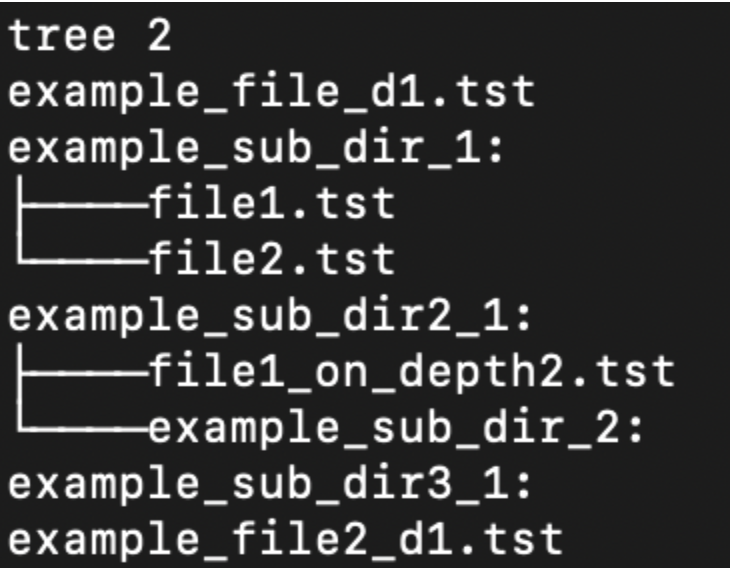
\includegraphics[scale=0.8]{Resources/tree.png}}
\end{figure}





\subsubsection*{{\titr arman}}
\addcontentsline{toc}{subsubsection}{{\fehrestContent arman}}

این قسمت امکان انتقال خروجی یک دستور به عنوان یکی از ورودی‌های دستور بعدی را فراهم می‌کند. به این ترتیب خروجی دستور قبلی به عنوان ورودی --str دستور بعدی در صورت وجود استفاده می‌شود. برای استفاده از این قابلیت بین دو دستور علامت =D قرار می‌گیرد.\\

\textbf{مثال}\\

فرض کنید قبل از اجرای دستور، فایل a.txt یک فایل خالی است.


\begin{mybox}[colback=yellow]{مثال}
	\begin{latin}	
		tree 2 =D insertstr --file a.txt --pos 1:0
	\end{latin}
\end{mybox}

\newpage
بعد از اجرای این دستور محتوای فایل a.txt عبارت است از:\\

\begin{latin}
// a.txt\\
├── example\_file2\_d1.tst\\
├── example\_file\_d1.tst\\
├── example\_sub\_dir\_1\\
│   ├── file1.tst\\
│   └── file2.tst\\
├── example\_sub\_dir2\_1\\
│   ├── example\_sub\_dir\_2\\
│   └── file1\_on\_depth2.tst\\
└── example\_sub\_dir3\_1\\
\end{latin}

دقت کنید که به عنوان دستور اول قبل از علامت arman همه دستوراتی که خروجی می‌دهند می‌توانند قرار گیرند. این دستورات عبارتند از grep, cat, find, tree و ...\\

همچنین به عنوان دستور دوم بعد از علامت arman تمامی دستوراتی که ورودی رشته می‌گیرند و یا به عبارت دیگر در آن دستورات --str مشهود است می‌تواند قرار گیرد. در واقع این دستورات به عنوان دستور دوم می‌آیند و اما دیگر --str در آن دستور نمی‌آید و برنامه شما باید به صورت خودکار خروجی دستور قبلی را به عنوان ورودی رشته به دستور جدید بدهد. در مثال بالا این موضوع مشهود است.


































% دستورات هر منو فقط داخل آن‌ها معتبر است و اگر در منوی مربوطه صدا زده نشوند، 
% باید خطای مناسب چاپ شود.

% \subsubsection*{{\titr دستورات مرتبط با منو}}
% \addcontentsline{toc}{subsubsection}{{\fehrestContent دستورات مرتبط با 
% منو}}
% \vspace{.5cm}
% \textbf{ورود به یک منو:}
% \begin{mybox}[colback=yellow]{مثال}
% 	\begin{latin}	
% 		menu enter <menu name>
% 	\end{latin}
% \end{mybox}


% در صورتی که کاربر داخل یک منوی دیگر باشد باید خطای زیر چاپ شود:
% \\
% \begin{mybox}[colback=yellow]{پیغام به کاربر}
% 	\begin{latin}	
% 		menu navigation is not possible
% 	\end{latin}
% \end{mybox}

% \vspace{.5cm}
% \textbf{خروج از یک منو:}
% \begin{mybox}[colback=yellow]{دستور}
% 	\begin{latin}	
% 		menu exit
% 	\end{latin}
% \end{mybox}
% در صورتی داخل یک منو باشیم، این دستور ما را به منوی بالاتر می‌برد و اگر در 
% منوی اصلی باشیم وارد منوی ورود و ثبت‌نام خواهیم شد. در صورتی که در منوی 
% ورود 
% و ثبت‌نام بودیم، بازی خاتمه خواهد یافت.

% \vspace{.5cm}
% \newpage
% \textbf{منوی فعلی:}
% \begin{mybox}[colback=yellow]{دستور}
% 	\begin{latin}	
% 		menu show-current 
% 	\end{latin}
% \end{mybox}
% این دستور نام منوی فعلی را نشان می‌دهد و اگر در منوی اصلی باشیم 
% \lr{Main Menu} و اگر در منوی ورود و ثبت‌نام باشیم \lr{Login Menu} چاپ می‌شود.

% \vspace{.5cm}
% \textbf{ساخت کاربر جدید:}
% \begin{mybox}[colback=yellow]{دستور}
% 	\begin{latin}	
% 		user create -{}-username <username> -{}-nickname <nickname> 
% 		-{}-password 
% 		<password>
% 	\end{latin}
% \end{mybox}
% پیغام موفقیت:
% \begin{mybox}[colback=yellow]{پیغام به کاربر}
% 	\begin{latin}	
% 		user created successfully!
% 	\end{latin}
% \end{mybox}
% خطا‌های زیر در صورت وجود به همین ترتیب بررسی شوند:
% \\
% نام کاربری تکراری:
% \begin{mybox}[colback=yellow]{پیغام به کاربر}
% 	\begin{latin}	
% 		user with username <username> already exists
% 	\end{latin}
% \end{mybox}
% نام مستعار تکراری:
% \begin{mybox}[colback=yellow]{پیغام به کاربر}
% 	\begin{latin}	
% 		user with nickname <nickname> already exists
% 	\end{latin}
% \end{mybox}

% \vspace{.5cm}
% \textbf{ورود کاربر:}
% \begin{mybox}[colback=yellow]{دستور}
% 	\begin{latin}	
% 		user login -{}-username <username> -{}-password <password>
% 	\end{latin}
% \end{mybox}
% پیغام موفقیت:
% \begin{mybox}[colback=yellow]{پیغام به کاربر}
% 	\begin{latin}	
% 		user logged in successfully!
% 	\end{latin}
% \end{mybox}
% خطا‌های زیر در صورت وجود به همین ترتیب بررسی شوند:
% \\
% عدم وجود کاربر با این نام کاربری:
% \begin{mybox}[colback=yellow]{پیغام به کاربر}
% 	\begin{latin}	
% 		Username and password didn’t match!
% 	\end{latin}
% \end{mybox}
% رمز اشتباه:
% \begin{mybox}[colback=yellow]{پیغام به کاربر}
% 	\begin{latin}	
% 		Username and password didn’t match!
% 	\end{latin}
% \end{mybox}
% توجه کنید که از دیدگاه امنیت، یک تلاش ناموفق برای ورود هیچ‌گاه نباید دارای 
% اطلاعاتی باشد که فرایند ورود را برای بار دوم راحت‌تر کند. مثلا اگر فردی 
% صرفا 
% قصد دزدیدن یکسری اکانت بدون توجه به صاحب آن‌ها را داشته باشد و در نتیجه 
% یکسری نام‌کاربری تصادفی را امتحان کند، در صورتی که نام‌کاربری و پسورد مطابقت 
% نداشت، نباید از پیام ما متوجه بشود که نام‌کاربری که وارد کرده، واقعا در 
% سیستم وجود دارد. در نتیجه در هر دو حالت بالا پیغام خطای یکسانی چاپ می‌شود.

% \vspace{.5cm}
% \textbf{خروج کاربر:}
% \begin{mybox}[colback=yellow]{دستور}
% 	\begin{latin}	
% 		user logout
% 	\end{latin}
% \end{mybox}
% این دستور تنها در منوی اصلی معتبر است و در صورت موفقیت، وارد منوی ورودی و 
% ثبت‌نام می‌شود.
% \\
% پیغام موفقیت:
% \begin{mybox}[colback=yellow]{پیغام به کاربر}
% 	\begin{latin}	
% 		user logged out successfully!
% 	\end{latin}
% \end{mybox}

% \vspace{.5cm}
% \textbf{بازی:}
% \\
% همانطور که گفته شد، این بازی یک بازی چند نفره است، لذا شما باید یوزرنیم افرادی که میخواهید با آن‌ها بازی کنید را داشته باشید تا به صورت زیر وارد بازی شوید.\\

% \begin{mybox}[colback=yellow]{دستور}
% 	\begin{latin}	
% 		play game -{}-player1 <username> -{}-player2 <username>
% 	\end{latin}
% \end{mybox}
% \newpage
% \noindent \textbf{دقت کنید} اگر تعداد افرادی که قرار بود با آن‌ها بازی کنید، بیشتر بود، نیاز است که به همین ترتیب در دستور شروع بازی، ابتدا \lr{-{}-player} و سپس شماره آن بازیکن و سپس بعد از آن یوزرنیم آن را وارد کنید.\\
%  در صورتی که یک یا چند یوزرنیم وجود نداشت پیغام خطای مناسب به کاربر نشان داده شود. و همینطور در صورت ورود به بازی نیز پیغام مناسب چاپ شود.\\
% \vspace{.5cm}
% \textbf{پروفایل:}
% \\
% پس از ورود به منوی profile دستورات زیر معتبر هستند:
% \\
% \\
% \vspace{.5cm}
% \textbf{تغییر نام مستعار:}
% \begin{mybox}[colback=yellow]{دستور}
% 	\begin{latin}	
% 		profile change -{}-nickname <nickname>
% 	\end{latin}
% \end{mybox}
% پیغام موفقیت:
% \begin{mybox}[colback=yellow]{پیغام به کاربر}
% 	\begin{latin}	
% 		nickname changed successfully!
% 	\end{latin}
% \end{mybox}
% در صورتی که کاربری با این نام مستعار وجود داشت خطای زیر چاپ شود:
% \begin{mybox}[colback=yellow]{پیغام به کاربر}
% 	\begin{latin}	
% 		user with nickname <nickname> already exists
% 	\end{latin}
% \end{mybox}

% \vspace{.5cm}
% \textbf{تغییر رمز عبور:}
% \begin{mybox}[colback=yellow]{دستور}
% 	\begin{latin}	
% 		profile change -{}-password -{}-current <current password> -{}-new <new 
% 		password>
% 	\end{latin}
% \end{mybox}
% پیغام موفقیت:
% \begin{mybox}[colback=yellow]{پیغام به کاربر}
% 	\begin{latin}	
% 		password changed successfully!
% 	\end{latin}
% \end{mybox}
% خطا‌های زیر در صورت وجود به همین ترتیب بررسی شوند:
% \\
% نادرست بودن رمز فعلی:
% \begin{mybox}[colback=yellow]{پیغام به کاربر}
% 	\begin{latin}	
% 		current password is invalid
% 	\end{latin}
% \end{mybox}
% یکی بودن رمز قدیم و جدید:
% \begin{mybox}[colback=yellow]{پیغام به کاربر}
% 	\begin{latin}	
% 		please enter a new password
% 	\end{latin}
% \end{mybox}

% \newpage 
% \subsection*{{\titr نقشه بازی}}
% \addcontentsline{toc}{subsection}{{\fehrestContent نقشه بازی}}
% پیشنهاد ما این است که نقشه‌ی کوچکی در ترمینال خود نمایش دهید، و با هر دستور جدید این نقشه را بروز کنید و بعد از ابتدا چاپ کنید.

% نقشه‌ی شما می‌تواند عنصرهای مختلف درون نقشه را به صورت رنگ، حروف اختصاری، و یا کلمات کامل نشان دهد. همچنین می‌توانید برخی از اطلاعات را به زمان انتخاب شدن یک کاشی واگذار کنید. پیشنهاد می‌شود که مختصات هر خانه را چاپ کنید تا انتخاب یک خانه‌ی خاص در دستورات ممکن باشد.
% مثلا یک نقشه‌ی ممکن می‌تواند مانند شکل زیر باشد:
% \begin{figure}[H]
%     \centerline{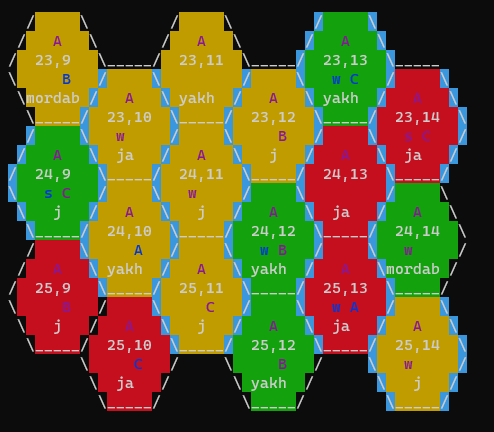
\includegraphics[scale=0.8]{Resources/map.png}}
% \end{figure}
% به طور مثال کاشی بالا سمت چپ نقشه، در مختصات 23,9 قرار دارد. این کاشی در محدوده‌ی مرزهای تمدن \lr{A} (با رنگ بنفش) است، در زمین صحرایی (با توجه به رنگ زرد پس‌زمینه‌ی آن)  واقع شده و ویژگی مرداب را دارا است. در این خانه یک یگان نظامی از نوع \lr{Ballista} قرار دارد که مربوط به تمدنی‌ست که رنگ آبی را دارد (حرف \lr{B})، اما یگان غیرنظامی‌ای در آن وجود ندارد. در ضلع پایین سمت راست این کاشی، یک رودخانه واقع شده است که با رنگ پس‌زمینه‌ی آبی مشخص شده است.
% از طرف دیگر، کاشی پایینی آن در مختصات 24,9 در زمین علفزار (با توجه به رنگ سبز پس‌زمینه‌ی آن) قرار دارد. در این کاشی که از ویژگی جنگل (با توجه به حرف \lr{j}) برخوردار است، یک یگان غیرنظامی مهاجر متعلق به تمدن آبی (با توحه به حرف \lr{s}) و با توجه به حرف \lr{C} یک واحد نظامی \lr{Catapult} متعلق به تمدن بنفش (همان \lr{A}) قرار دارد.
% شما باید نقشه‌ای مثل شکل بالا ایجاد کنید. البته شما در انتخاب این که چطور می‌خواهید اطلاعات درون نقشه را نشان دهید، مختارید. مثلا می‌توانید رودخانه‌ها را به جای رنگ پس‌زمینه، با مرزهای «-» برای کاشی نشان دهید. یا به جای استفاده از رنگ پس‌زمینه برای نشان دادن نوع زمین، این اطلاعات را به طور مستقیم روی نقشه بنویسید. آن‌چه که در نهایت اهمیت دارد این است که \textbf{وضعیت رودخانه‌ها، مالکیت زمین‌ها، یگان‌های موجود در کاشی و مالکیت آن‌ها، مختصات کاشی، نوع زمین کاشی، ویژگی زمین کاشی، منبع موجود در کاشی و پیشرفت‌های موجود در کاشی  در نقشه مشخص باشد.}

% \subsection*{\titr کد تقلب}
% \addcontentsline{toc}{subsection}{{\fehrestContent کد تقلب}}
% احتمالا در بازی های زیادی دیدید (شنیدید) که یک سری کدهای تقلب وجود دارد که بازی را از حالت عادی خارج می‌کند، نمونه ای از این کد ها مثلا در بازی GTA وجود دارد، می‌تواند باعث شود تمامی اسلحه‌ها برای بازکن در دسترس باشد، یا در مثال دیگر می‌تواند باعث شوند بازیکن هیچگاه جان خودش را از دست ندهد. در پروژه شما نیز این قابلیت باید پیاده سازی شود. در این حالت پروژه شما باید بتواند کارهایی که در حالت عادی نمی‌توانید انجام دهد را پیاده سازی کند، نمونه ای از این کار‌ها را می‌توان افزایش پول به مقدار دلخواه، گذشتن چند نوبت پشت سر هم، پیروزی در یک نبرد، به دست اوردن غذا و تکنولوژی و ... باشد. در اینجا نمونه‌ای از دستورات پیشنهادی را برای شما آورده‌ایم. شما نیز می‌توانید خودتان دستورات دیگری برای این حالت توسعه دهید و در زمینه های دیگر استفاده کنید. (دقت کنید برای تمام فعالیت‌های بازی اعم از برد یک دست بازی، حرکت یگان‌ها، ساختمان‌ها، یونیت‌ها، شهرها و... کد تقلب داشته باشید.)\\
% جلو رفتن نوبت‌های بازی:
% \begin{mybox}[colback=yellow]{دستور}
% 	\begin{latin}	
% 		increase --turn <amount>
% 	\end{latin}
% \end{mybox}
% زیاد شدن پول:
% \begin{mybox}[colback=yellow]{دستور}
% 	\begin{latin}	
% 		increase --gold <amount>
% 	\end{latin}
% \end{mybox}

% \subsection*{\titr مواردی که باید در فاز 1 پیاده سازی شوند}
% \addcontentsline{toc}{subsection}{{\fehrestContent پیاده سازی فاز 1}}
% برای راحتی کار شما، در فاز اول، یک سری موارد کلی ای از بازی پیاده سازی می‌شوند که در واقع همان منطق اصلی بازی هستند، و سایر موارد به ترتیب در فازهای بعدی پروژه تکمیل می‌شوند.\\
% علاوه بر موارد مخصوص به فاز 1 که در همین داک دیدید (منوها، نقشه بازی، کدهای تقلب) شما باید مواردی از داک بازی نیز که مربوط به فاز 1 هست را نیز پیاده سازی کنید.\\
% در واقع بازی پیاده سازی شده در فاز 1 به شکلی به طور کلی اینگونه می‌باشد:\\
% کاربران می‌توانند برای خودشان یک سری یوزر در بازی بسازند، اطلاعاتشان را عوض کنند، با سایر کاربران بازی کنند. در محیط بازی نیز در فاز 1 شما باید زمین‌ها، ویژگی‌های آن‌ها، یگان‌ها، منابع، حرکت یگان‌ها بر روی زمین، منابع، تکنولوژی را داشته باشید. در فاز 1 برد و باخت یک تمدن  حمله کردن تمدن‌ها و یگان‌های نظامی به یکدیگر چک نمی‌شوند و شما باید آن‌ها را در فازهای بعدی پروژه تکمیل کنید.\\
% به طور کلی‌تر، موارد زیر را نیاز نیست در فاز 1 پیاده سازی کنید:
% \begin{itemize}
%     \item برخی از اعمال تمدن‌ها (معامله کردن با یک تمدن دیگر، جنگ)
%     \item برد و باخت در بازی
%     \item خرابه‌ها(ruins)
%     \item ساختمان‌ها
% \end{itemize}

% \section*{\titr چک پوینت}
% \addcontentsline{toc}{section}{{\fehrestContent چک پوینت}}

% یکی از مواردی که در این پروژه باید به آن دقت کنید، چک پوینت‌ها هستند. در واقع چک پوینت‌ها همان ددلاین‌های تقسیم شده در طول هر فاز می‌باشند. از شما خواسته می‌شود با توجه به زمان پایان هر چک پوینت، مواردی از فاز اول پروژه که در آن چک پوینت باید زده شوند را، با تگ "\lr{CP\#.0.0}" در مخزن گیت‌هاب خود قرار دهید.\\
% در این فاز، شما 2 چک پوینت و یک ددلاین پایانی فاز 1 را دارید. همچنین هر چک پوینت نیز میزان نمره‌ای از کل نمره پروژه دارد.\\
% مواردی که باید تا پایان زمان هر چک پوینت زده شوند در زیر آمده است.

% \newpage
% \subsection*{\titr چک پوینت 1}
% \addcontentsline{toc}{subsection}{{\fehrestContent چک پوینت 1}}
% \begin{itemize}
%     \item حجم موارد خواسته شده در این چک پوینت نسبت به کل مطالب این فاز: 40\%
%     \\
%     \\
% کامل کردن منو ها (تمپلیت) و قابلیت ساخت اکانت وجود دیتابیس \lr{User}ها  و پیاده کردن Map بازی و معماری(لزومی به پیاده سازی کامل نیست صرفا تقریبا مشخص باشد چه تابعایی و چه چیزهایی لازم است) و کلاس های لازم برای Object های اولیه مثل Block - City - Unit پیاده سازی Movement and Exploration ( توانایی حرکت دادن نیرو ها در MAP و war of fog ) هر نوع نیرو یک کلاس پدر Unit دارد و توانایی دستور دادن به این کلاس کلی مد نظر است (پیاده سازی نیروهای جنگی در ادامه)
% \end{itemize}

% \subsection*{\titr چک پوینت 2}
% \addcontentsline{toc}{subsection}{{\fehrestContent چک پوینت 2}}
%   \begin{itemize}  
%     \item حجم موارد خواسته شده در این چک پوینت نسبت به کل مطالب این فاز: 30\%
%     \\
%     \\
%     قابلیت احداث شهر و منطق مربوط به شهرها
% \end{itemize}
% \subsection*{\titr فاز 1}
% \addcontentsline{toc}{subsection}{{\fehrestContent فاز 1}}
%  \begin{itemize}   
%     \item حجم موارد خواسته شده در این چک پوینت نسبت به کل مطالب این فاز: 30\%
%     \\
%     \\
%     موارد باقی مانده از پیاده سازی فاز اول پروژه
% \end{itemize}




\end{document}







